\chapter{CI/CD and release engineering}

\section{Engineering principles}

A coding agent belongs upstream of protected merge and deployment gates. CI validates candidate commits, not the conversation that produced them. Required checks, review rules and deployment permissions must be administered outside the worker identity. Workflow configuration from untrusted branches can execute arbitrary code if the runner is not appropriately isolated.\src{G2,G3}

\section{Implementation approach}

Use separate workflows for untrusted pull request verification and privileged release. Give the verification job read-only repository permissions and no production secrets. Pin actions by immutable commit and review dependency updates. Run trusted checks, upload bounded evidence and require status checks plus independent review on protected branches. Use a separate release identity and approval environment for production.

\section{Verification and limitations}

Test a rejected candidate and prove that an agent identity cannot bypass required checks, edit protection rules or deploy. The example workflow uses a toy trusted test suite and requires stronger repository-level protections before production use.

Figure~\ref{fig:d18} illustrates the conceptual flow from Candidate commit to Release approval. The edges describe the proposed integration or control relationship, not undocumented internal calls.

\begin{figure}[htbp]\centering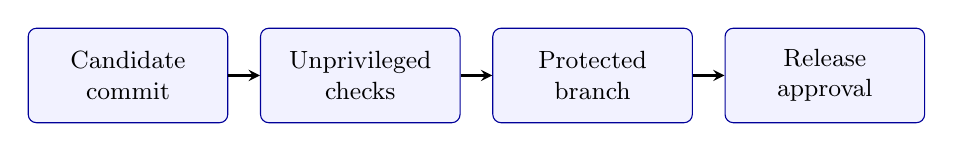
\begin{tikzpicture}[nodebox/.style={draw=blue!60!black,fill=blue!5,rounded corners=3pt,minimum height=12mm,text width=23mm,align=center,font=\small},>=stealth]
\node[nodebox] (n0) at (0.00,0.00) {Candidate commit};
\node[nodebox] (n1) at (2.95,0.00) {Unprivileged checks};
\node[nodebox] (n2) at (5.90,0.00) {Protected branch};
\node[nodebox] (n3) at (8.85,0.00) {Release approval};
\draw[->,thick] (n0.east) -- (n1.west);
\draw[->,thick] (n1.east) -- (n2.west);
\draw[->,thick] (n2.east) -- (n3.west);
\end{tikzpicture}
\caption{CI/CD integration (conceptual view).}\label{fig:d18}\end{figure}

\section{Chapter conclusion}

Apply the stated verification criteria before expanding the scope of this workflow. Record deviations, evidence and unresolved risks in the task record.
